\documentclass[a4paper, english, 12pt]{article} % norsk & english is supported

\newcommand{\exerciseNumber}{2}
\newcommand{\solutions}{true} % Change to   true   to create solutions
% Must be defined before course package, \exerciseNumber, and \solutions
\usepackage{IMF}

\usepackage{MA0301}

\graphicspath{{./images/}} %Path to images

\begin{document}

\titlebox

\seksjon{2.2}

\begin{problem}[19]
  Provide the steps and reasons, as in Exercise 18, to establish the following
  logical equivalences
\end{problem}

\begin{subproblem}[3]
  $[(\neg p \vee \neg q) \to (p \wedge q \wedge r)] \ \Leftrightarrow p \wedge q$
\end{subproblem}

\begin{answer}  
  \begin{align*}
                    \ & [(\neg p \vee \neg q) \to (p \wedge q \wedge r)]
                      && \textbf{Reasons}\\
    \Leftrightarrow \ & \neg (\neg p \vee \neg q) \vee  (p \wedge q \wedge r)
                      && \text{Material implication $a\to b \Leftrightarrow \neg a \vee b$}\\
    \Leftrightarrow \ &  (p \wedge q) \vee  (p \wedge q \wedge r)
                      && \text{DeMorgan's Laws and Law of Double Negation}\\
    \Leftrightarrow \ &  (p \wedge q)
                      && \text{Absorption laws and associative properties of $\vee$}.
  \end{align*}
\end{answer}

\begin{problem}
  Simplify each of the networks shown in \cref{fig:diagrams}.
\end{problem}

\begin{answer}
  For \cref{fig:truth-diagram-1} notice that the first block $r \vee t \vee \neg
  r$ is true when $r$ is either true or false, in other words the block is
  always true. Similarly $\neg r \vee q \vee \neg q$ is always true. Thus, the
  diagram simplifies to $p \vee \neg q$ as shown in \cref{fig:solution-1}.

  Imagine walking from $T_0$ to $T_1$ in \cref{fig:truth-diagram-2}, there is no
  way to do this without passing through both $p$ and $q$. All the other boolean
  variables can be avoided and thus, are not necceccary. The resulting diagram
  is shown in \cref{fig:solution-2}.
\end{answer}

\begin{figure}[hbp!]
  \centering
  \begin{subfigure}[b]{0.45\textwidth}
    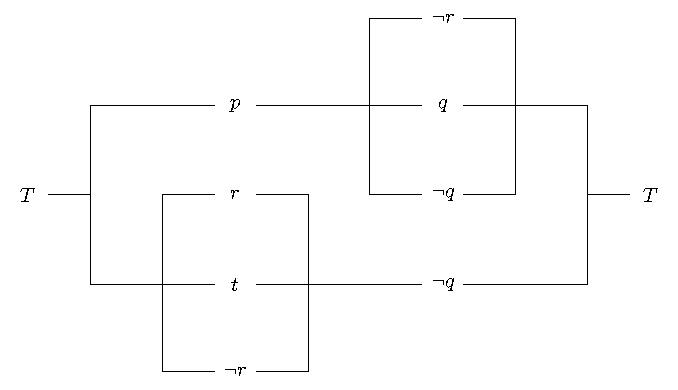
\includegraphics[width=\textwidth]{MA0301-oving-02-truth-diagram-1}
    \caption{}
    \label{fig:truth-diagram-1}
  \end{subfigure}
  ~ %add desired spacing between images, e. g. ~, \quad, \qquad, \hfill etc. 
  % (or a blank line to force the subfigure onto a new line)
  \begin{subfigure}[b]{0.5\textwidth}
    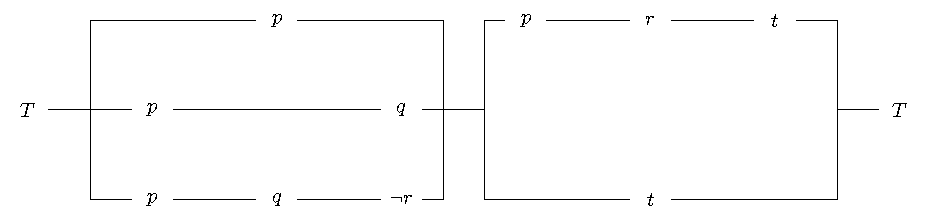
\includegraphics[width=\textwidth]{MA0301-oving-02-truth-diagram-2}
    \caption{}
    \label{fig:truth-diagram-2}
  \end{subfigure}
  \caption{}\label{fig:diagrams}
\end{figure}

\begin{answer}
  \begin{figure}[hbp!]
    \centering
    \begin{subfigure}[b]{0.45\textwidth}
      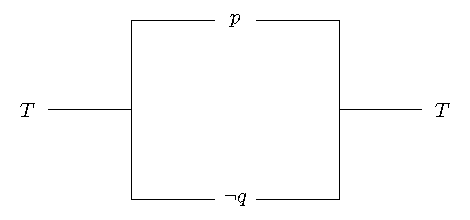
\includegraphics[width=\textwidth]{MA0301-oving-02-truth-diagram-1-solution}
      \caption{}
      \label{fig:solution-1}
    \end{subfigure}
    ~ %add desired spacing between images, e. g. ~, \quad, \qquad, \hfill etc. 
    % (or a blank line to force the subfigure onto a new line)
    \begin{subfigure}[b]{0.5\textwidth}
      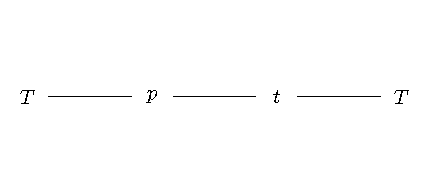
\includegraphics[width=\textwidth]{MA0301-oving-02-truth-diagram-2-solution}
      \caption{}
      \label{fig:solution-2}
    \end{subfigure}
    \caption{}\label{fig:truth-diagrams-solutions}
  \end{figure}
\end{answer}


\seksjon{2.3}

\begin{problem}[2]
  Use truth tables to verify that each of the following is a logical implication
\end{problem}

\begin{subproblem}[2]
  $[(p \to q) \wedge \neg q] \to \neg p$
\end{subproblem}
  
\begin{answer}
  \begin{table}[htbp!]
    \centering
    \begin{tabular}{L L L L L L L}
      \toprule
      p & q & \neg q & & (p \to q) \wedge \neg q & [(p \to q) \wedge \neg q ] \to \neg p \\
      \midrule
      \F & \F & \T & \T & \T & \T \\
      \F & \T & \F & \T & \F & \T \\ 
      \T & \F & \T & \F & \F & \T \\
      \T & \T & \F & \T & \F & \T \\
      \bottomrule
    \end{tabular}
  \end{table}
\end{answer}
  
\begin{subproblem}[4]
  $[(p \to r) \wedge (q \to r)] \to [(p \vee q) \to r]$
\end{subproblem}
  
\begin{answer}
  \begin{table}[htbp!]
    \centering
    \begin{tabular}{L L L L L L L}
      \toprule
      p & q & r & p \to r & q \to r & (p \vee q) \to r & [(p \to r) \wedge (q \to r)] \to [(p \vee q) \to r] \\
      \midrule
      \F & \F & \F & \T & \T & \T & \T \\
      \F & \F & \T & \T & \T & \T & \T \\
      \F & \T & \F & \T & \F & \F & \T \\
      \F & \T & \T & \T & \T & \T & \T \\
      \T & \F & \F & \F & \T & \F & \T \\
      \T & \F & \T & \T & \T & \T & \T \\
      \T & \T & \F & \F & \F & \F & \T \\
      \T & \T & \T & \T & \T & \T & \T \\
      \bottomrule
    \end{tabular}
  \end{table}
\end{answer}

\begin{problem}[8]
  Give the reasons for the steps verifying the following argument.
  %
  \begin{align*}
    & (\neg p \vee q) \to r \\
    & r \to (s \vee t) \\ 
    & \neg s \wedge \neg u \\
    & \neg u \to \neg t \\[-0.5cm]
    \cmidrule{1-2} \\[-1cm]
     \therefore & \ p
  \end{align*}
\end{problem}

\begin{tabular}{r l p{1cm} l}
  \textbf{Steps} & & & \textbf{Reasons} \\
  \ITEM \label{step-1}& $\neg s \wedge \neg u$
        & & \ans{Premisse}\\
  \ITEM & $\neg u$
        & & \ans{\Cref{step-1} and the rule of Conjunctive Simplification}\\
  \ITEM \label{step-3} & $\neg u \to \neg t$
        & & \ans{Premisse}\\
  \ITEM \label{step-4} & $\neg t$
        & & \ans{\Cref{step-3} and Modus Potens}\\
  \ITEM \label{step-5} & $\neg s$
        & & \ans{\Cref{step-1} and the rule of Conjunctive Simplification}\\
  \ITEM \label{step-6} & $\neg s \wedge \neg t$
        & & \ans{\Cref{step-4,step-5} and the Rule of Conjunction}\\
  \ITEM & $r \to (s \vee t)$
        & & \ans{Premisse}\\
  \ITEM \label{step-8} & $\neg (s \vee t) \to \neg r$
        & & \ans{\Cref{step-8} and Contraposition $a \to b \Leftrightarrow \neg b \to \neg a$} \\
  \ITEM \label{step-9} & $(\neg s \wedge \neg t) \to \neg r$
        & & \ans{\Cref{step-9} and DeMorgan's Laws}\\
  \ITEM & $\neg r$
        & & \ans{\Cref{step-6,step-9} and Modus Potens}\\
  \ITEM \label{step-11} & $(\neg p \vee q) \to r$
        & & \ans{Premisse}\\
  \ITEM \label{step-12} & $\neg r \to \neg (\neg p \vee q)$
        & & \ans{\Cref{step-11} and Contraposition $a \to b \Leftrightarrow \neg b \to \neg a$}\\
  \ITEM \label{step-13} & $\neg r \to (p \wedge \neg q)$
        & & \ans{\Cref{step-12} and DeMorgan's Laws}\\
  \ITEM \label{step-14} & $p \wedge \neg q$
        & & \ans{\Cref{step-13} and Modus Potens}\\
  \ITEM & $\therefore p$
        & & \ans{\Cref{step-14} and the rule of Conjunctive Simplification}
\end{tabular}
  
\seksjon{2.4}

\begin{problem}[8]
  Let $p(x)$, $q(x)$, and $r(x)$ denote the following open statements.
  %
  \begin{align*}
    p(x) & \colon \quad x^2 - 8x + 15 = 0 \\
    q(x) & \colon \quad x \text{ is odd} \\
    r(x) & \colon \quad x > 0
  \end{align*}
  %
  For the universe of all integers, determine the truth or falsity of each of
  the following statements. If a statement is false, give a counterexample.
\end{problem}

\begin{subproblem}[5]
  $\exists \, x \ [p(x) \to q(x)]$
\end{subproblem}
%
\begin{answer} 
  \paragraph{True:} As $p(x) = (x-3)(x-5)$ we have $p(x) = 0 \Leftrightarrow x =
  3 \wedge x = 5$. Thus, there exists a solution to $p(x)$ such that $x$ is odd.
  %
\end{answer}

\begin{subproblem}
  $\forall \, x \ [\neg q(x) \to \neg p(x)]$
\end{subproblem}
  %
\begin{answer}
  \paragraph{True:} $q(x) \vee \neg p(x)$. As every solution to $p(x)$ is odd,
  every even $x$ implies that $x$ is \emph{not} an solution to $p(x)$. Thus, the
  statement above holds.
\end{answer}
  %
\begin{subproblem}
  $\exists \, x \ [p(x) \to (q(x) \wedge r(x))]$
\end{subproblem}
  %
\begin{answer}
  \paragraph{True:} As $p(5)$ is True, there exists some solution to $p(x)$ such that $x$ is
  positive and odd.
\end{answer}
  %
\begin{subproblem}
  $\forall \, x \ [(p(x) \vee q(x)) \to r(x)]$
\end{subproblem}
  %
\begin{answer}
  \paragraph{False: } Let $x$ be a negative even number. Then $p(x) \vee q(x)$
  is False, but $r(x)$ is True.
\end{answer}


  
\begin{problem}[12]
  \begin{subproblem}
    Let $p(x,y)$ denote the open statement ``$x$ divides $y$'', where the
    universe for each of the variables $x$, $y$ comprises all integers.
    Determine the truth value of each of the following statements; if a
    quantified statement is false, provide an explanation or a counterexample.
  \end{subproblem}
\end{problem}
% 
\begin{subsubproblem}[3]
  $\forall \, y \ p(1, y)$
\end{subsubproblem}

\begin{answer}
  \paragraph{True:} As $y/1 = 1$ for all $y$.
\end{answer}
    
\begin{subsubproblem}
  $\forall \, x \ p(x, 0)$
\end{subsubproblem}

\begin{answer}
  \paragraph{False:} take $x = 0$ as an counterexample $p(0,0)$ is false as $0/0$ is undefined.
\end{answer}
    
\begin{subsubproblem}[6]
  $\forall \, y \ \exists \,  x \ p(x,y)$
\end{subsubproblem}

\begin{answer}
  \paragraph{True:} This is ``obviously'' true? For every $y$ let $x=1$, then $p(1,y)$ is true for
  all $y$.
\end{answer}
    
\begin{subsubproblem}
  $\exists y \ \forall \, x \ p(x, y)$
\end{subsubproblem}

\begin{answer}
  \paragraph{False: } Let $x = 0$ then $p(0, y)$ is undefined for all $y$.
\end{answer}
    
    
\begin{subsubproblem}
  $\forall \, x \ \forall \, y \ [(p(x, y) \wedge p(y, x)) \to (x = y)]$
\end{subsubproblem}

\begin{answer}
  \paragraph{False:} Let $x = y = 0$. Then $x = y$, but $p(x,y)$ is undefined
  and thus, $p(x,y) \wedge p(y,x)$ is false. If we exclude $0$ the statement holds.
\end{answer}
  %
\begin{subproblem}[3]
  Let $p(x,y)$ denote the open statement''$x$ divides $y$``, as before, but let
  the universe now be compromised of the \emph{positive} integers $x$, $y$.
  Determine the truth value of each of the following statements. If the
  statement is false, provide an explanation or a counterexample.
\end{subproblem}
% 
\begin{subsubproblem}
  $\forall \,x \ \exists\, y \ p(x, y)$
\end{subsubproblem}

\begin{answer}
  \paragraph{True:} Let $y = x$, as $x, y > 0$ we can always choose such an $y$.
\end{answer}
    
\begin{subsubproblem}
  $\forall \,y \ \exists\, x \ p(x, y)$
\end{subsubproblem}
\begin{answer}
  \paragraph{True} We could let $x = 1$ here as well, but this states that the
  $x$ can be different for every $y$. To illustrate this let $x = y$. Then
  clearly $p(x,y)=p(y,y)$ is true as $y/y$. Thus, for every $y$ we can find an
  $x$ such that $p(x,y)$ is true.
\end{answer}

\begin{subsubproblem}
  $\exists \,x \ \forall \, y \ p(x, y)$
\end{subsubproblem}
\begin{answer}
  \paragraph{True:} Again let $x = 1$, then $p(x,y)=p(1,y)$ is true, as $y/1 =
  y$. 
\end{answer}

\begin{subsubproblem}
  $\exists \,y \ \forall \, x \ p(x, y)$
\end{subsubproblem}
\begin{answer}
  \paragraph{False:} This asks whether there exists a single number $y$ that
  divides every $x$. Meaning $y$ has to divide $1$, $2$ and so forth. If such a
  number where to exist it would have to be the product of all the integers 
 \begin{equation*}
   y = 1 \cdot 2 \cdot 3 \cdots = \prod_{i \in \mathbb{N}} i\,.
 \end{equation*}
 Then clearly $y$ divides $x$ for every integer $x > 0$, however $y$ is now no longer
 an integer!
\end{answer} 

\end{document}